% \chapter{Theoretical Background}
\chapter{Methodology and Model Validation}


This chapter presents the design of the feed antenna and the antenna lens in Ansys HFSS, together with the methodology used to validate the resulting MIMO channel model. Validation is carried out across three solvers drawn from two simulation platforms: Sionna-RT, a ray-tracing-based channel simulator; HFSS SBR+, which approximates propagation through high-frequency ray tracing and reports the channel in terms of S-parameters; and HFSS Hybrid, which combines the finite element method (FEM) with SBR+ ray tracing and likewise reports the channel through S-parameters. Each solver is evaluated under an identical $3\times3$ MIMO configuration, with particular emphasis on how the channel varies across the angular domain, so that the resulting channel-quality trends can be compared consistently across solvers.

\section{Antenna}
\subsection{Antenna Model}
In free space, the electric far field radiated by a transmit antenna can be described as a spherical wave originating from the antenna's phase center \cite{NVIDIACorporation2026}:
\begin{equation}
\mathbf{E}_T(r, \theta_T, \varphi_T) = \sqrt{\frac{P_T G_T Z_0}{2\pi}} \frac{e^{-jk_0 r} }{r}\mathbf{F}_T(\theta_T, \varphi_T)
\end{equation}

This formulation is closely related to the classical far-field expression derived from the antenna's current distribution and vector effective length \cite{ConstantineABalanis2016}, but is instead expressed in terms of input power and gain. The parameters are defined as follows: $P_T$ is the input power delivered to the transmitting antenna; $G_T$ is its maximum gain; $Z_0$ is the free-space impedance; $\mathbf{F}_T$ is the complex vector field pattern of the antenna; the factor $1/r$ accounts for spherical spreading loss; and $e^{-jk_0 r}$ represents the propagation phase delay.

Assuming conjugate impedance matching, the input power $P_T$ delivered to an antenna with impedance $Z_T$, fed by a voltage source of complex amplitude $V_T$, is given by \cite{NVIDIACorporation2026}:
\begin{equation}
P_T = \frac{|V_T|^2}{8\Re\{Z_T\}}
\end{equation}

At the receiver, the transmitted field $\mathbf{E}_T(r)$ arrives as a locally planar incoming wave $\mathbf{E}_R$, incident on the receiving antenna from the direction $(\theta_R, \varphi_R)$. The corresponding open-circuit voltage $V_R$ induced at the antenna terminals is given by \cite{NVIDIACorporation2026}:
\begin{equation}
V_R = \sqrt{\frac{\lambda^2}{4\pi} G_R \frac{4\Re\{Z_R\}}{Z_0}} \mathbf{F}_R(\theta_R, \varphi_R)^\text{H} \mathbf{E}_R,
\end{equation}
where $\lambda$ is the wavelength; $G_R$ is the gain of the receiving antenna; $Z_R$ is its impedance; $Z_0$ is the free-space impedance; $\mathbf{F}_R$ is the complex vector field pattern of the receiving antenna; and the superscript $\text{H}$ denotes the Hermitian (conjugate) transpose, which accounts for the polarization overlap between the incoming wave and the receiving antenna.

When the polarization of the incoming wave matches that of the receiving antenna, this expression reduces to the absolute voltage magnitude:
\begin{equation}
\label{eq:VR_matched}
|V_\text{R}| = \sqrt{\frac{\lambda^2}{4\pi} G_R \frac{4\Re\{Z_\text{R}\}}{Z_0}} \|\mathbf{F}_\text{R}(\theta_\text{R}, \varphi_\text{R})\| \|\mathbf{E}_\text{R}\|.
\end{equation}

Substituting the matched-polarization voltage of \eqref{eq:VR_matched} into the standard power relation, the available received power at the output of the receiving antenna can be expressed as:
\begin{align}
    P_\text{R} &= \frac{|V_\text{R}|^2}{8\Re\{Z_\text{R}\}} \\
    &= \left(\frac{\lambda}{4\pi r}\right)^2 G_\text{R} G_\text{T} P_\text{T} \left|\mathbf{F}_\text{R}(\theta_\text{R}, \varphi_\text{R})^{\mathsf{H}} \mathbf{F}_\text{T}(\theta_\text{T}, \varphi_\text{T})\right|^2.
\end{align}
% \begin{equation}
%     P_\text{R} = \left(\frac{\lambda}{4\pi r}\right)^2 G_\text{R} G_\text{T} P_\text{T} \left|\mathbf{F}_\text{R}(\theta_\text{R}, \varphi_\text{R})^{\mathsf{H}} \mathbf{F}_\text{T}(\theta_\text{T}, \varphi_\text{T})\right|^2.
% \end{equation}

\subsection{Antenna Design}
In this thesis, a patch antenna is used as the feed antenna behind the antenna lens. Figure~\ref{fig:patch_antenna_design} shows the simulated return loss of the patch antenna together with its design geometry and the corresponding simulated field distribution.

\begin{figure}[htbp]
    \centering
    \begin{minipage}{0.48\textwidth}
        \centering
        
\includegraphics[width=\linewidth]{AntennaPatch_ReturnLoss.PNG}
        (a)
    \end{minipage}
    \hfill
    \begin{minipage}{0.48\textwidth}
        \centering
        
\includegraphics[width=\linewidth]{AntennaPatch_Design_Fields.PNG}
        (b)
    \end{minipage}
    \caption{Patch feed antenna: (a) simulated return loss $|S_{11}|$; (b) antenna design geometry with simulated field distribution.}
    \label{fig:patch_antenna_design}
\end{figure}

For the Monte Carlo simulation, an omnidirectional (wire/monopole) antenna is used instead, so that the transmitter radiates uniformly across the randomized user positions.
% TODO: add return loss and radiation pattern figures for the omnidirectional antenna.

\section{Antenna Lens Design}
Antenna Lens Design is built on the Metasurface Transmitarray Lens Design. Also basic Theory about it.

\subsection{Metasurface Unit-Cell Design}
    \begin{figure}[htbp]
        \centering
        \begin{minipage}{0.3\textwidth}
            \centering
            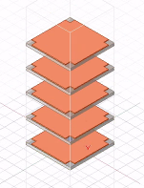
\includegraphics[width=\linewidth]{Images/Unitcell_Design.png}
            (a)
            % \label{fig:unitcell}
        \end{minipage}
        \begin{minipage}{0.48\textwidth}
            \centering
            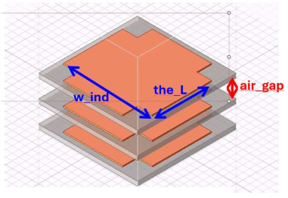
\includegraphics[width=\linewidth]{Images/Unitcell_Design_geometry.png}
            (b)
            % \label{fig:geometry}
        \end{minipage}
        \hfill        
        \caption{Unitcell design (a)5 layers with 1mm airgap (b)Sweep dimension}
        \label{fig:UnitcellDesign}
    \end{figure}
    The unit cell design is adopted from prior work on broadband metasurface superstrates, which enables polarization-independent wave focusing and gain enhancement at Ka-band frequencies\cite{Lee2022}. As shown in Figure \ref{fig:UnitcellDesign}, the unit cell consists of a 5-layer stacked structure separated by air gaps, where the geometrical parameters such as patch width and layer spacing are varied to control the transmission response. 

    To evaluate the unit cell performance, a periodic simulation setup with Floquet ports is employed, as illustrated in Figure \ref{fig:UnitcellDesign}. This configuration allows the extraction of transmission characteristics under plane wave excitation.

    % \centering
\begin{figure}[htbp]
     \begin{minipage}{0.24\textwidth}
         \centering
         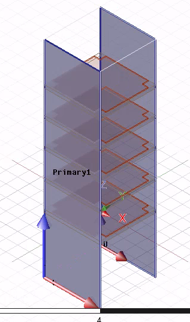
\includegraphics[width=\linewidth]{Images/FloqBoundary-1.png}
        %  \caption{Bloch Boundary 1}
        (a)
         \label{fig:floq_bound1}
     \end{minipage}
     \hfill
     \begin{minipage}{0.24\textwidth}
         \centering
         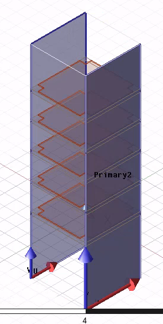
\includegraphics[width=\linewidth]{Images/FloqBoundary-2.png}
        %  \caption{Bloch Boundary 2}
        (b)
         \label{fig:floq_bound2}
     \end{minipage}
     \hfill
     \begin{minipage}{0.24\textwidth}
         \centering
         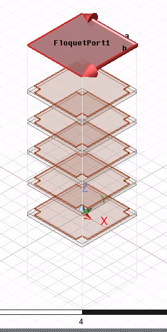
\includegraphics[width=\linewidth]{Images/FloqPort-1.png}
        %  \caption{Floquet Port 1}
         \label{fig:floq_port1}
         (c)
     \end{minipage}
     \hfill
     \begin{minipage}{0.24\textwidth}
         \centering
         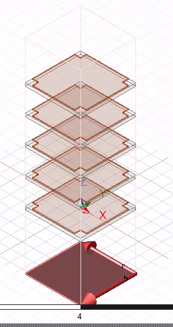
\includegraphics[width=\linewidth]{Images/FloqPort-2.png}
        %  \caption{Floquet Port 2}
         \label{fig:floq_port2}
         (d)
     \end{minipage}
     \caption{Simulation Setup Unit cell with FloquetPort}
     \label{fig:floquet_setup}
\end{figure}


    Using this simulation setup, the unit cell is optimized with respect to its transmission coefficient. As illustrated in Figure~\ref{fig:floquet_setup}, a range of geometrical variations is explored, and the final design is selected such that $S_{21}>-5\text{\,dB}$ at 38 GHz, thereby ensuring sufficient transmission efficiency for the lens application.

    This selection criterion follows directly from the power conservation principle\,[2]: the power incident on the unit cell must be fully accounted for by the reflected, transmitted, and dissipated components, as expressed in Equation~\ref{eq:power_conservation},
    \begin{equation}
        \left|S_{11}\right|^{2}+\left|S_{21}\right|^{2}+P_{loss}=1.
        \label{eq:power_conservation}
    \end{equation}
    From this relation, the transmitted and reflected power fractions can be expressed directly in terms of the simulated S-parameters as
    \begin{align}
        P_{T} &= \left|S_{21}\right|^{2} = 10^{\frac{S_{21,\text{dB}}}{10}}, \\
        P_{R} &= \left|S_{11}\right|^{2} = 10^{\frac{S_{11,\text{dB}}}{10}},
        \label{eq:power_definitions}
    \end{align}
    where the notation used above is summarized as follows:
    \begin{itemize}
        \item $S_{21}$: Transmission coefficient (forward transmission)
        \item $S_{11}$: Reflection coefficient (input reflection)
        \item $\left|S_{21}\right|^{2}$: Transmitted power ratio
        \item $\left|S_{11}\right|^{2}$: Reflected power ratio
        \item $S_{21,\text{dB}}$, $S_{11,\text{dB}}$: S-parameters in dB scale
        \item $P_{T}$: Transmitted power
        \item $P_{R}$: Reflected power
        \item $P_{\text{loss}}$: Power loss due to dielectric and conductor losses
    \end{itemize}
    Together, these relations justify the $S_{21}>-5\text{\,dB}$ criterion adopted above, as they guarantee that reflection and dissipative loss remain sufficiently small for the unit cell to operate efficiently as a transmitting element.

    \begin{figure}[htbp]
        \centering
        \begin{minipage}{\textwidth}
            \centering
            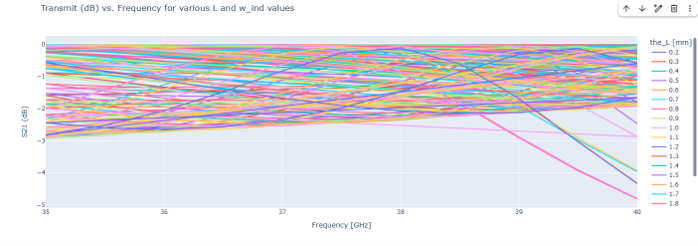
\includegraphics[width=\linewidth]{Images/UnitCell_Magnitude.png}
            % (a)
            
        \end{minipage}
        \hfill        
        \begin{minipage}{\textwidth}
            \centering
            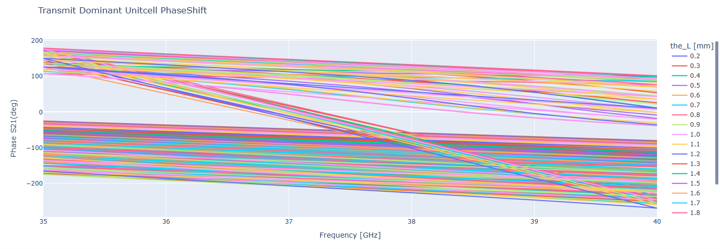
\includegraphics[width=\linewidth]{Images/UnitCell_Phase.png}
            % (b)
            % \caption{Transmission Phase}
            % \label{fig:UnitCell_Phase}
        \end{minipage}
        \caption{Transmit S21 in dB and phase shift angle deg.  with various dimension of unitcell}
            \label{fig:Unitcell_profile}
    \end{figure}

\subsection{Lens Phase Distribution / Cell Arrangement}

The working principle of the antenna lens is based on compensating the phase difference of a spherical wavefront.
When a point source is located at the focal point, the wave arriving at the lens aperture has different path lengths. To convert this into a planar wave, the lens must introduce a compensating phase \cite{Al-Joumayly2011}, \cite{RezkiElArif2023}:
    \begin{equation}
        \phi(x,y) = \frac{2\pi}{\lambda_{0}}\left(\sqrt{(x-x_{f})^{2}+(y-y_{f})^{2}+f^{2}} - f\right) + \phi_{\text{init}}
        \label{eq:phase_profile}
    \end{equation}

    \noindent where:
    \begin{itemize}
        \item $\phi(x,y)$: Required phase at position $(x,y)$
        \item $(x,y)$: Unit cell coordinates
        \item $(x_{f},y_{f})$: Center of the aperture
        \item $f$: Focal distance
        \item $\lambda_{0}$: Free-space wavelength
        \item $\phi_{\text{init}}$: Initial phase offset
    \end{itemize}
This equation ensures that all transmitted waves are in-phase, producing a collimated beam.
The metasurface antenna lens is designed with the following parameters:

\begin{table}[h!]
	\begin{center}
		\caption{Design parameters of the metasurface antenna lens}
		\label{table:lens_design_parameters}
		\begin{tabular}{|l|c|}
			\hline
			\textbf{Parameter} & \textbf{Value} \\
			\hline
			Antenna array size & $20 \times 20$ \\
			Antenna dimension & $44.24\,\text{mm} \times 44.24\,\text{mm}$ (@$2.367\,\text{mm} \times 2.367\,\text{mm}$ per unit cell) \\
			Number of layers & 5 \\
			Target focal point & 30\,mm \\
            Actual focal point & 14\,mm \\
			\hline
		\end{tabular}
	\end{center}
\end{table}

The required phase is implemented in a discrete manner across the aperture, where each unit cell represents a specific phase value.
As shown in Figure 4, the phase distribution forms a concentric (radial) pattern, indicating proper compensation of the spherical wavefront from the focal point. The symmetry also confirms that the phase is correctly centered. This phase distribution has been matched to the explored unit cell database to ensure practical realizability.
Furthermore, Figure 5 illustrates the physical realization of this phase distribution on the transmitarray structure, where each unit cell geometry corresponds to its assigned phase based on the explored unit cell responses.
Overall, the implemented phase profile closely follows the theoretical design, with minor deviations due to discretization.

% gambar Phase Distribution Phasenya
% <Tambahkan Gambar Antenna Lens>

\subsection{Focal Characteristics}
% To validate the designed transmitarray metasurface lens, a plane-wave incidence simulation is performed to assess its focusing performance under a realistic excitation scenario.

% As illustrated in Figure~6, the metasurface is illuminated by a normally incident plane wave, with the propagation vector $\mathbf{k}$ oriented perpendicular to the lens aperture and the electric field $\mathbf{E}_{0}$ polarized orthogonal to $\mathbf{k}$, thereby ensuring uniform excitation across the entire unit-cell array.

% <Gambar Setup Test Simulation>

% The resulting transmitted field distribution is then examined to evaluate the focusing performance of the lens. As shown in Figure~7, the transmitted electric field is concentrated along the propagation axis and converges toward the target focal region, indicating that the incident plane wave is successfully focused by the metasurface.

% Taken together, these results confirm that the phase distribution obtained from the explored unit-cell database is correctly realized by the transmitarray structure, yielding the intended focusing behavior and validating the overall lens design methodology.

% <Gambar Hasil Simulation>

The lens was designed for a target focal distance of $f=30\,\mathrm{mm}$ using the phase profile of Equation~\ref{eq:phase_profile}, but the full-wave simulation in Figure~\ref{fig:focal_point_verification} shows the field lobes contracting to their tightest point at approximately $14\,\mathrm{mm}$, considerably closer than the design target. This shift is attributed to phase quantization: the continuous phase required by Equation~\ref{eq:phase_profile} can only be approximated by the finite set of phase states available from the explored unit-cell database, so the design focal length should be treated as the target used to generate the phase mask, while $14\,\mathrm{mm}$ is the actual focal distance of the realized transmitarray.

\begin{figure}[htbp]
    \centering
    
\includegraphics[width=0.7\linewidth]{AntennaLens20x20_VerifFocalPoint.png}
    \caption{Simulated E-field distribution of the $20\times20$ antenna lens, used to verify the location of the actual axial focal point}
    \label{fig:focal_point_verification}
\end{figure}

To further characterize the focusing behavior of the lens, its response is evaluated under oblique plane-wave incidence, with the incident angle swept from $0^\circ$ to $-60^\circ$ in steps of $15^\circ$. Figure~\ref{fig:focal_characteristics} shows the resulting field-intensity distribution behind the lens aperture for each incident angle.

\begin{figure}[htbp]
    \centering
    \begin{minipage}{0.19\textwidth}
        \centering
        
\includegraphics[width=\linewidth]{FocalCharacter_0deg.png}
        (a) $0^\circ$
    \end{minipage}
    \hfill
    \begin{minipage}{0.19\textwidth}
        \centering
        
\includegraphics[width=\linewidth]{FocalCharacter_m15degdeg.png}
        (b) $-15^\circ$
    \end{minipage}
    \hfill
    \begin{minipage}{0.19\textwidth}
        \centering
        
\includegraphics[width=\linewidth]{FocalCharacter_m30deg.png}
        (c) $-30^\circ$
    \end{minipage}
    \hfill
    \begin{minipage}{0.19\textwidth}
        \centering
        
\includegraphics[width=\linewidth]{FocalCharacter_m45deg.png}
        (d) $-45^\circ$
    \end{minipage}
    \hfill
    \begin{minipage}{0.19\textwidth}
        \centering
        
\includegraphics[width=\linewidth]{FocalCharacter_m60deg.png}
        (e) $-60^\circ$
    \end{minipage}
    \caption{Focal-plane field-intensity distribution behind the antenna lens for plane-wave incidence at (a) $0^\circ$, (b) $-15^\circ$, (c) $-30^\circ$, (d) $-45^\circ$, and (e) $-60^\circ$}
    \label{fig:focal_characteristics}
\end{figure}

At normal incidence ($0^\circ$), the focal spot is formed directly on-axis behind the lens, consistent with the boresight focusing behavior discussed above. As the incident angle becomes more oblique, the focal spot progressively shifts away from the boresight axis while remaining at approximately the same radial distance from the lens, so that the locus of focal points traced across the angular sweep forms a focal arc rather than a fixed focal point. This behavior is expected for a transmitarray lens with a fixed phase profile: because the phase mask is optimized for a single design incidence direction, illuminating the lens from other angles causes the focus to relocate along this arc instead of staying fixed in space. The results in Figure~\ref{fig:focal_characteristics} also show that the sharpness of the focal spot degrades as the incident angle increases, with the response at $-30^\circ$ to $-60^\circ$ exhibiting more diffuse and multiple intensity peaks and stronger side-lobe energy compared with the well-defined single focal spot at $0^\circ$ and $-15^\circ$. This indicates that, while the lens is capable of focusing incident waves arriving from a range of angles along a focal arc, its focusing quality is best near the design incidence direction and degrades progressively toward wider oblique angles.

\subsection{Antenna Radiation Test}

Before presenting the simulated results, it is useful to recall the acquisition model underlying the transmitarray far-field pattern. Figure~\ref{fig:transmitarray_coord_system} defines the coordinate system: the feed is located at position vector $\vec{r}_f$ and illuminates the $(m,n)$-th transmitarray element at $\vec{r}_{mn}$ with feed-incidence angle $\theta_f(m,n)$, while the far-field is observed along the direction $\hat{\boldsymbol{u}}$, making angle $\theta_e$ with the array normal, relative to the main-beam direction $\hat{\boldsymbol{u}}_0$. Under this geometry, the complex far-field pattern of an $M\times N$ transmitarray is given by
\begin{equation}
    \begin{aligned}
        E(\theta,\varphi)
        &= \sum_{m=1}^{M}\sum_{n=1}^{N}
        \cos^{q_e}(\theta)\,
        \frac{\cos^{q_f}\!\left(\theta_f(m,n)\right)}
        {\left|\vec{r}_{mn}-\vec{r}_{f}\right|} \\[4pt]
        &\quad \times
        \exp\!\left\{-jk\left(
        \left|\vec{r}_{mn}-\vec{r}_{f}\right|
        -\vec{r}_{mn}\cdot\hat{\boldsymbol{u}}
        \right)\right\}
        \left|T_{mn}\right|e^{j\psi_{mn}},
    \end{aligned}
    \label{eq:transmitarray_pattern}
\end{equation}
where $\theta$ and $\varphi$ specify the observation direction $\hat{\boldsymbol{u}}$; $q_e$ and $q_f$ control the element and feed pattern factors, respectively; $k=2\pi/\lambda$ is the free-space wavenumber; and $|T_{mn}|e^{j\psi_{mn}}$ is the complex transmission coefficient (magnitude and phase) applied by the $(m,n)$-th element. The total radiation pattern is thus the coherent sum of every element's contribution, each weighted by its feed illumination, its own element/feed pattern factors, the free-space path loss $1/\left|\vec{r}_{mn}-\vec{r}_{f}\right|$, and the propagation phase accumulated from the feed to the element and from the element toward the observation direction. This model is the basis on which the HFSS-simulated RX lens patterns discussed below are interpreted.

\begin{figure}[htbp]
    \centering
    
\includegraphics[width=0.6\linewidth]{AntennaLensRadiationPatternAsset/TransmitArray_CoorSystem.PNG}
    \caption{Coordinate system used for the transmitarray far-field acquisition model, showing the feed, the $(m,n)$-th element, and the observation direction relative to the main-beam direction $\hat{\boldsymbol{u}}_0$}
    \label{fig:transmitarray_coord_system}
\end{figure}

The receive (RX) lens element is further characterized through its far-field radiation pattern, extracted directly from HFSS far-field data at $f=38~\mathrm{GHz}$ for six representative steering states: $-45^\circ$, $0^\circ$, $+15^\circ$, $+30^\circ$, $+45^\circ$, and $+60^\circ$. Because the responses at $\pm15^\circ$, $\pm30^\circ$, and $\pm60^\circ$ are mirror-symmetric about boresight, only one sign is reported for each of these magnitudes, whereas both signs are reported at $45^\circ$ since they correspond to two distinct simulated configurations; a dedicated symmetry check on the world-frame boresight azimuth confirms $\mathrm{az}_{+}\approx-\mathrm{az}_{-}$ to within $0.01^\circ$ for every magnitude, validating that the lens steers symmetrically about boresight. For all six configurations, the computed radiation efficiency remains in the low-$90\%$ range, consistent with genuine (lossy) HFSS data rather than a numerical artifact.

Figure~\ref{fig:radiation_pattern_3d} shows the normalized 3D radiation pattern (40~dB dynamic range) for each steering state, while Figure~\ref{fig:radiation_pattern_vertical_cut} overlays the corresponding full $360^\circ$ vertical (X-Z plane) gain cuts on a shared polar axis. The main lobe is clearly visible and well-formed in every case, and its pointing direction shifts progressively with the steering angle: the peak elevation angle $\theta_{\mathrm{peak}}$ moves from $90^\circ$ (broadside) at $0^\circ$ steering down to about $38^\circ$ at $+60^\circ$ steering. This confirms, from the antenna-pattern side, the same beam-steering behavior already inferred from the focal-arc analysis in the preceding subsection, while also showing that side-lobe levels grow moderately at the larger steering angles ($\pm45^\circ$, $\pm60^\circ$), mirroring the degradation in focal-spot sharpness observed earlier.

\begin{figure}[htbp]
    \centering
    
\includegraphics[width=0.95\linewidth]{AntennaLensRadiationPatternOutput/matlab_visualization/figures/matlab_radiation_pattern_3d_all_patterns.png}
    \caption{Normalized 3D far-field radiation patterns (40~dB dynamic range) of the RX lens element for steering angles of $-45^\circ$, $0^\circ$, $+15^\circ$, $+30^\circ$, $+45^\circ$, and $+60^\circ$}
    \label{fig:radiation_pattern_3d}
\end{figure}

\begin{figure}[htbp]
    \centering
    
\includegraphics[width=0.75\linewidth]{AntennaLensRadiationPatternOutput/vertical_cut_360/figures/vertical_cut_360_all_patterns.png}
    \caption{Full $360^\circ$ vertical gain cut (X-Z plane) of the RX lens element overlaid across all evaluated steering angles, showing the progressive shift of the main-lobe pointing direction with steering angle}
    \label{fig:radiation_pattern_vertical_cut}
\end{figure}

\section{MIMO Channel Modeling}

Place $N_R$ Receiver Antenna and $N_T$ Transmitter Antenna in free space. Receiver Antenna observe signal $y_i$ that construct by acumulated of many Transmitter signal $\mathbf{x}$ over medium between which called channel$\mathbf{H}$ including noise$\mathbf{n}$ . Then this system model can written as :
\begin{equation}
    \mathbf{y} = \mathbf{H}\mathbf{x} + \mathbf{n}
    \label{eq:basicMimo}
\end{equation}

this Basic system model can represent in many MIMO scheme including MIMO angular domain\cite{Tse2005}\cite{Challita2022}. In this thesis will try formulation on angular domain with scheme Receiver place on focal-plane behind antenna lens system ristic. Then we compare it conventional coplanar configuration.

\subsection{Singular Value Decomposition}
At every evaluated frequency, the $3\times3$ channel matrix $\mathbf{H}$ obtained from Equation~\ref{eq:basicMimo} is decomposed using the singular value decomposition (SVD)
\begin{equation}
    \mathbf{H} = \mathbf{U}\boldsymbol{\Sigma}\mathbf{V}^{H},
    \qquad
    \boldsymbol{\Sigma} = \operatorname{diag}(\sigma_1,\sigma_2,\sigma_3),
    \qquad
    \sigma_1\geq\sigma_2\geq\sigma_3\geq0,
    \label{eq:mimo_svd}
\end{equation}
where $\mathbf{U}$ and $\mathbf{V}$ are unitary matrices whose columns form the receive- and transmit-side eigenmode bases, and $\sigma_1,\sigma_2,\sigma_3$ are the singular values of $\mathbf{H}$. Each singular value corresponds to the gain of one independent spatial eigenchannel that can, in principle, carry an independent data stream. Whenever only the relative spatial structure of the channel is of interest, $\mathbf{H}$ is additionally evaluated after Frobenius normalization,
\begin{equation}
    \widetilde{\mathbf{H}} = \frac{\mathbf{H}}{\lVert\mathbf{H}\rVert_{\mathrm{F}}},
    \label{eq:mimo_frobenius_normalization}
\end{equation}
which rescales all three singular values by the same factor and therefore removes the overall link-budget difference between the with-lens and without-lens cases while leaving their relative proportions, and hence the condition number and effective rank defined below, unchanged.

\subsection{Channel Quality Metrics}
Two scalar indicators are used to summarize how balanced the three singular values are. The condition number is the ratio of the largest to the smallest singular value,
\begin{equation}
    \kappa = \frac{\sigma_1}{\sigma_3},
    \label{eq:mimo_condition_number}
\end{equation}
so that $\kappa=1$ corresponds to three perfectly balanced spatial modes, while $\kappa\gg1$ indicates that the channel is dominated by a single mode. The effective rank is obtained by first normalizing the singular values by their total power,
\begin{equation}
    p_i = \frac{\sigma_i^{2}}{\sum_{k=1}^{3}\sigma_k^{2}},
    \qquad i=1,2,3,
    \label{eq:mimo_power_fraction}
\end{equation}
and then computing the exponential of the Shannon entropy of this power distribution,
\begin{equation}
    r_{\mathrm{eff}} = \exp\!\left(-\sum_{i=1}^{3}p_i\ln p_i\right),
    \qquad 1\leq r_{\mathrm{eff}}\leq3.
    \label{eq:mimo_effective_rank}
\end{equation}
An effective rank close to $1$ indicates that the channel is effectively rank-deficient and dominated by a single eigenmode, whereas a value close to $3$ indicates that all three spatial modes contribute comparable power, which is the condition required for full spatial multiplexing. Because $\kappa$ and $r_{\mathrm{eff}}$ depend only on the ratios between singular values, they take identical values whether they are computed from the raw channel $\mathbf{H}$ or the Frobenius-normalized channel $\widetilde{\mathbf{H}}$ of Equation~\ref{eq:mimo_frobenius_normalization}.

\subsection{Channel Correlation Matrix}
The spatial correlation between antenna elements is quantified from the receive- and transmit-side Gram matrices of the channel,
\begin{equation}
    \mathbf{R}_{\mathrm{RX}} = \mathbf{D}_{\mathrm{RX}}^{-1/2}\,\mathbf{H}\mathbf{H}^{H}\,\mathbf{D}_{\mathrm{RX}}^{-1/2},
    \qquad
    \mathbf{R}_{\mathrm{TX}} = \mathbf{D}_{\mathrm{TX}}^{-1/2}\,\mathbf{H}^{H}\mathbf{H}\,\mathbf{D}_{\mathrm{TX}}^{-1/2},
    \label{eq:mimo_correlation_matrix}
\end{equation}
where $\mathbf{D}_{\mathrm{RX}}$ and $\mathbf{D}_{\mathrm{TX}}$ are diagonal matrices containing the receive- and transmit-side element powers, so that $\mathbf{R}_{\mathrm{RX}}$ and $\mathbf{R}_{\mathrm{TX}}$ have unit diagonal entries and off-diagonal entries equal to the normalized cross-correlation between antenna pairs. The channel is summarized by the mean and maximum magnitude of the off-diagonal entries of $\mathbf{R}_{\mathrm{RX}}$ and $\mathbf{R}_{\mathrm{TX}}$, reported separately for the receive and transmit sides. A smaller off-diagonal correlation indicates that the antenna elements observe more statistically independent channels, which is favorable for spatial multiplexing, whereas a correlation approaching unity indicates that the elements are close to indistinguishable from one another.

\subsection{Channel Capacity}
Assuming equal power allocation across the transmit antennas and spatially white receiver noise, the ergodic MIMO capacity at linear SNR $\rho$ is
\begin{equation}
    C(\rho) = \log_2\det\!\left(\mathbf{I}_{3} + \frac{\rho}{N_T}\mathbf{H}\mathbf{H}^{H}\right)
    = \sum_{i=1}^{3}\log_2\!\left(1+\frac{\rho}{N_T}\sigma_i^{2}\right)
    \quad\text{bps/Hz},
    \label{eq:mimo_capacity}
\end{equation}
with $N_T=3$ transmit antennas. Unless otherwise stated, the capacity results reported in this thesis are evaluated at $\rho=100$, corresponding to a $20~\mathrm{dB}$ operating SNR. Because capacity in Equation~\ref{eq:mimo_capacity} depends on the absolute singular values rather than only their ratios, it is, unlike $\kappa$ and $r_{\mathrm{eff}}$, sensitive to the Frobenius normalization of Equation~\ref{eq:mimo_frobenius_normalization}: the capacity computed from the raw channel $\mathbf{H}$ reflects both the spatial-mode balance and the absolute link budget, while the capacity computed from $\widetilde{\mathbf{H}}$ isolates the contribution of the spatial-mode balance alone by removing the difference in overall channel strength between the with-lens and without-lens cases.

\section{HFSS-Based Electromagnetic Simulation}
This section focuses on the electromagnetic simulation carried out in Ansys HFSS, whose raw output takes the form of measured S-parameters rather than a direct channel matrix. Accordingly, the generic MIMO system model of Equation~\ref{eq:basicMimo} is reformulated below in terms of S-parameters, giving the S-parameter-based channel evaluation used throughout the HFSS results in this chapter.

\subsubsection{S-Parameter-Based Communication Channel Evaluation}

In this work, the measured S-parameters are used to construct an empirical frequency-domain communication channel.
For each frequency point, the MIMO channel matrix is defined as
\begin{equation}
    \mathbf{H}(f) \in \mathbb{C}^{N_R \times N_T},
\end{equation}
where \(N_R\) is the number of receive ports and \(N_T\) is the number of transmit ports.
Each element of the channel matrix is obtained from the measured transmission coefficient between the corresponding transmit and receive ports:
\begin{equation}
    H_{ij}(f) = S(\mathrm{rx}_i,\mathrm{tx}_j;f),
\end{equation}
where \(S(\mathrm{rx}_i,\mathrm{tx}_j;f)\) denotes the complex S-parameter from the \(j\)-th transmit port to the \(i\)-th receive port at frequency \(f\).

For the \(3 \times 3\) measurement configuration used in this work, the channel matrix is written as
\begin{equation}
\mathbf{H}(f)
=
\begin{bmatrix}
S(\mathrm{rx1},\mathrm{tx1}) & S(\mathrm{rx1},\mathrm{tx2}) & S(\mathrm{rx1},\mathrm{tx3}) \\
S(\mathrm{rx2},\mathrm{tx1}) & S(\mathrm{rx2},\mathrm{tx2}) & S(\mathrm{rx2},\mathrm{tx3}) \\
S(\mathrm{rx3},\mathrm{tx1}) & S(\mathrm{rx3},\mathrm{tx2}) & S(\mathrm{rx3},\mathrm{tx3})
\end{bmatrix}.
\end{equation}

The physical meaning of each index in $\mathbf{H}(f)$ is summarized in Table~\ref{tab:sparam_index_mapping}: the receive ports $\mathrm{rx1}$--$\mathrm{rx3}$ are fixed observation points behind the antenna lens along its focal arc, while the transmit ports $\mathrm{tx1}$--$\mathrm{tx3}$ each face their corresponding receive port from a radius much larger than the lens focal length, so that the illuminating wavefront approaches a locally plane wave and the $3\times3$ evaluation emphasizes the incident angle rather than the exact TX-to-lens distance.

\begin{table}[h!]
    \centering
    \caption{Angular position and role of each receive and transmit index used in $\mathbf{H}(f)$}
    \label{tab:sparam_index_mapping}
    \begin{tabular}{|l|c|l|}
        \hline
        \textbf{Index} & \textbf{Angular Position} & \textbf{Description} \\
        \hline
        $\mathrm{rx1}$ & $0^\circ$ & Central focal receiver \\
        $\mathrm{rx2}$ & $+45^\circ$ & Positive-angle focal receiver \\
        $\mathrm{rx3}$ & $-45^\circ$ & Negative-angle focal receiver \\
        \hline
        $\mathrm{tx1}$ & $0^\circ$ & Facing $\mathrm{rx1}$, far radius \\
        $\mathrm{tx2}$ & $+45^\circ$ & Facing $\mathrm{rx2}$, far radius \\
        $\mathrm{tx3}$ & $-45^\circ$ & Facing $\mathrm{rx3}$, far radius \\
        \hline
    \end{tabular}
\end{table}

Under this convention, the diagonal entries $S(\mathrm{rx}_i,\mathrm{tx}_i)$ correspond to matched incident and observation directions, while the off-diagonal entries $S(\mathrm{rx}_i,\mathrm{tx}_j)$, $i\neq j$, correspond to the cross-angular response between mismatched incident and observation directions.

The corresponding frequency-domain input-output relation can be expressed as
\begin{equation}
    \mathbf{y}(f) = \mathbf{H}(f)\mathbf{x}(f) + \mathbf{n}(f),
\end{equation}
where
\begin{equation}
    \mathbf{x}(f) \in \mathbb{C}^{N_T \times 1}
\end{equation}
is the transmitted signal vector or incident-mode excitation vector,
\begin{equation}
    \mathbf{y}(f) \in \mathbb{C}^{N_R \times 1}
\end{equation}
is the received signal vector, and \(\mathbf{n}(f)\) denotes the additive noise vector.

It should be noted that \(\mathbf{H}(f)\) in this formulation represents a measured end-to-end RF channel response.
Therefore, it does not only describe the pure free-space propagation channel, but also includes the effects of the transmit antenna, receive antenna, lens response, propagation path, mutual coupling, impedance mismatch, and measurement reference plane.
Thus, the proposed formulation is more accurately described as an S-parameter-based empirical communication channel evaluation.

\subsection{Simulation Setup}
The electromagnetic simulation is carried out inside an indoor room environment measuring $3~\mathrm{m}\times5~\mathrm{m}\times3~\mathrm{m}$ (height $\times$ length $\times$ width), with the floor, ceiling, and all four walls assigned a concrete material to emulate a realistic indoor propagation environment with multipath reflections. The three-element receive antenna array, together with the antenna lens when present, is placed near one corner of the room, while the transmitter is positioned at a fixed distance along the room so that both line-of-sight and reflected propagation paths from the concrete boundaries are captured. Figure~\ref{fig:room_sbr} shows this room setup as used in the HFSS SBR+ solver, with the inset highlighting a close-up of the receive antenna array, and Figure~\ref{fig:room_hybrid} shows the equivalent setup used in the HFSS Hybrid solver, with the inset showing the close-up of the antenna lens together with the receive array and the transmit antenna.

\begin{figure}[htbp]
    \centering
    
\includegraphics[width=0.85\linewidth]{Room_SBR_withCloseup.png}
    \caption{Indoor room simulation environment ($3~\mathrm{m}\times5~\mathrm{m}\times3~\mathrm{m}$, concrete boundaries) used in the HFSS SBR+ solver, with a close-up of the receive antenna array}
    \label{fig:room_sbr}
\end{figure}

\begin{figure}[htbp]
    \centering
    
\includegraphics[width=0.85\linewidth]{Room_withCloseup.png}
    \caption{Indoor room simulation environment ($3~\mathrm{m}\times5~\mathrm{m}\times3~\mathrm{m}$, concrete boundaries) used in the HFSS Hybrid solver, with a close-up of the antenna lens and antenna array}
    \label{fig:room_hybrid}
\end{figure}

The detailed layout of the antenna array, the antenna lens, and the transmitter relative to the room is shown in Figures~\ref{fig:sbr_setup_detail}--\ref{fig:hybrid_setup_top_detail}. Figure~\ref{fig:sbr_setup_detail} shows the three-dimensional close-up used in the SBR+ solver, in which the three receive elements ($\mathrm{rx}_1$--$\mathrm{rx}_3$) and the three transmit elements ($\mathrm{tx}_1$--$\mathrm{tx}_3$) are arranged as separate radiating bodies without an explicit lens geometry. Figure~\ref{fig:sbr_setup_top_detail} shows the corresponding top-view schematic: the receive array is arranged on a focal arc in front of the antenna lens, with $\mathrm{rx}_1$ on boresight ($0^{\circ}$) and $\mathrm{rx}_2$ and $\mathrm{rx}_3$ offset by $+45^{\circ}$ and $-45^{\circ}$ about the lens focal point, respectively, while the three transmitters $\mathrm{tx}_1$--$\mathrm{tx}_3$ are placed on the opposite side of the lens along the transmitter-distance axis, each aimed back toward the receive array.

\begin{figure}[htbp]
    \centering
    
\includegraphics[width=0.6\linewidth]{SetupEnvirontment_SBR_WithLens.PNG}
    \caption{HFSS SBR+ solver: three-dimensional close-up of the receive array ($\mathrm{rx}_1$--$\mathrm{rx}_3$) and transmit array ($\mathrm{tx}_1$--$\mathrm{tx}_3$) with the antenna lens installed}
    \label{fig:sbr_setup_detail}
\end{figure}

\begin{figure}[htbp]
    \centering
    
\includegraphics[width=0.7\linewidth]{SetupEnvirontment_SBR_WithLens_TopDetails.PNG}
    \caption{HFSS SBR+ solver: top-view schematic showing the focal-arc placement of $\mathrm{rx}_1$ ($0^{\circ}$), $\mathrm{rx}_2$ ($+45^{\circ}$), and $\mathrm{rx}_3$ ($-45^{\circ}$) relative to the antenna lens, and the transmitter positions $\mathrm{tx}_1$--$\mathrm{tx}_3$}
    \label{fig:sbr_setup_top_detail}
\end{figure}

The same focal-arc arrangement is retained in the HFSS Hybrid solver, but with the antenna lens modeled explicitly as a multilayer dielectric structure rather than as an idealized ray-tracing object. Figure~\ref{fig:hybrid_setup_detail} shows the three-dimensional close-up of the multilayer lens together with the receive array on one side and the transmit antenna on the other, and Figure~\ref{fig:hybrid_setup_top_detail} shows the corresponding top-view schematic, confirming that the $0^{\circ}/{+45^{\circ}}/{-45^{\circ}}$ focal-arc geometry of $\mathrm{rx}_1$--$\mathrm{rx}_3$ and the transmitter-distance axis are consistent between the SBR+ and Hybrid setups.

\begin{figure}[htbp]
    \centering
    
\includegraphics[width=0.6\linewidth]{SetupEnvirontment__WithLens_Hybrid.jpeg}
    \caption{HFSS Hybrid solver: three-dimensional close-up of the multilayer antenna lens, receive array, and transmit antenna}
    \label{fig:hybrid_setup_detail}
\end{figure}

\begin{figure}[htbp]
    \centering
    
\includegraphics[width=0.6\linewidth]{SetupEnvirontment_WithLens_Hybrid_TopDetails.png}
    \caption{HFSS Hybrid solver: top-view schematic showing the focal-arc placement of $\mathrm{rx}_1$--$\mathrm{rx}_3$ relative to the multilayer antenna lens and the transmitter}
    \label{fig:hybrid_setup_top_detail}
\end{figure}

\subsection{HFSS SBR+ Solver}
\subsubsection{Channel Extraction Methodology}

The $3\times3$ MIMO channel is first extracted using the HFSS SBR+ (Shooting and Bouncing Ray) solver, which approximates wave propagation through high-frequency ray tracing. For each transmitter--receiver pair, the channel matrix $\mathbf{H}$ is evaluated at 37, 38, and 39 GHz, both with and without the antenna lens, so that the effect of the lens on the channel structure can be isolated.

In brief, SBR+ launches rays from the TX source and traces their reflection/transmission through the scene; at each hit point it applies the physical-optics (PO) approximation to obtain equivalent surface currents from the local incident, reflected, and transmitted fields, then radiates these currents to the RX side. The scattered field contributed by a ray footprint $S'$ is
\begin{equation}
    \bar{E}_s = \frac{1}{4\pi}\int_{S'} dS' \left[ (\hat{n}'\cdot\bar{E})\nabla'\frac{e^{-jkR}}{R} + (\hat{n}'\times\bar{E})\nabla'\frac{e^{-jkR}}{R} - j\omega\mu_0(\hat{n}'\times\bar{H})\nabla'\frac{e^{-jkR}}{R} \right],
    \label{eq:sbr_scattered_field}
\end{equation}
where $\bar{E}$ and $\bar{H}$ are the total surface fields at the hit point, $\hat{n}'$ is the surface normal, and $R$ is the distance to the observation point. This scattered field is converted into the S-parameter entry $S=b/a$ between the TX incident signal $a$ and the RX received signal
\begin{equation}
    b = \frac{-j\lambda}{\sqrt{4\pi\eta_0}}\,\bar{E}\cdot\bar{g}_{\text{Rx}},
    \label{eq:sbr_received_signal}
\end{equation}
with $\bar{g}_{\text{Rx}}$ the far-field polarized gain vector of the RX antenna, summed coherently over all ray paths reaching that RX to give the entry $S(\mathrm{rx}_i,\mathrm{tx}_j)$ of $\mathbf{H}(f)$.

\subsubsection{HFSS SBR+ Solver Results}
Figure~\ref{fig:sbr_power} shows the normalized power distribution across the $3\times3$ channel matrix. Without the lens, the transmitted power spreads almost uniformly across all transmitter--receiver pairs, e.g., at 38 GHz the diagonal terms $H(\mathrm{rx}_i,\mathrm{tx}_i)$ carry only 20.3--20.4\% of the received power each, while the off-diagonal terms still carry 1.2--9.1\%. With the lens installed, the power collapses strongly onto the diagonal: the $H(\mathrm{rx}_1,\mathrm{tx}_1)$ entry alone carries 53.4--69.7\% of the power over the 37--39 GHz band, while the off-diagonal entries fall to below 1.5\%. This confirms that the lens focuses each transmitter beam predominantly onto its corresponding receiver, suppressing unwanted coupling to the other receivers.

\begin{figure}[htbp]
    \centering
    
\includegraphics[width=0.85\linewidth]{channel_evaluation_per_method/HFSS_SBR+_Solver/power_distribution.png}
    \caption{HFSS SBR+ solver: normalized channel power distribution with and without the antenna lens}
    \label{fig:sbr_power}
\end{figure}

This diagonal focusing is also visible directly in the per-element magnitude response of Figure~\ref{fig:sbr_magnitude}: the co-located terms $H(\mathrm{rx}_1,\mathrm{tx}_1)$, $H(\mathrm{rx}_2,\mathrm{tx}_2)$, and $H(\mathrm{rx}_3,\mathrm{tx}_3)$ are enhanced by the lens by up to 9.1\,dB at 39 GHz, whereas the cross terms such as $H(\mathrm{rx}_1,\mathrm{tx}_3)$ are suppressed by as much as 15.6\,dB over the same band.

\begin{figure}[htbp]
    \centering
    
\includegraphics[width=0.85\linewidth]{channel_evaluation_per_method/HFSS_SBR+_Solver/channel_3x3_magnitude_db.png}
    \caption{HFSS SBR+ solver: $3\times3$ channel magnitude response with and without the antenna lens}
    \label{fig:sbr_magnitude}
\end{figure}

The resulting reduction in spatial correlation is quantified in Figure~\ref{fig:sbr_correlation}. Without the lens, the mean off-diagonal correlation is high, 0.71--0.81 on the receiver side and 0.71--0.81 on the transmitter side across 37--39 GHz, indicating a nearly rank-deficient, LoS-dominated channel. With the lens, the mean correlation drops to 0.18--0.27 (RX) and 0.16--0.25 (TX), showing that the lens substantially decorrelates the spatial channels.

\begin{figure}[htbp]
    \centering
    
\includegraphics[width=0.85\linewidth]{channel_evaluation_per_method/HFSS_SBR+_Solver/spatial_correlation.png}
    \caption{HFSS SBR+ solver: mean off-diagonal spatial correlation with and without the antenna lens}
    \label{fig:sbr_correlation}
\end{figure}

Table~\ref{table:sbr_metrics} summarizes the resulting MIMO channel-quality metrics at the design frequency of 38 GHz. Introducing the lens reduces the condition number from 6.25 to 2.22 and raises the effective rank from 1.61 to 2.36, close to the ideal value of 3 for a fully decorrelated $3\times3$ system. When the channel matrices are normalized to unit Frobenius norm to isolate the spatial-multiplexing gain from the difference in link budget, the capacity increases from 8.02 to 9.92\,bps/Hz.

\begin{table}[h!]
    \begin{center}
        \caption{HFSS SBR+ solver: MIMO channel-quality metrics at 38\,GHz}
        \label{table:sbr_metrics}
        \begin{tabular}{|l|c|c|}
            \hline
            \textbf{Metric} & \textbf{Without lens} & \textbf{With lens} \\
            \hline
            Condition number & 6.25 & 2.22 \\
            Effective rank & 1.61 & 2.36 \\
            Mean spatial correlation (RX / TX) & 0.77 / 0.77 & 0.21 / 0.19 \\
            Capacity, Frobenius-normalized (bps/Hz) & 8.02 & 9.92 \\
            \hline
        \end{tabular}
    \end{center}
\end{table}

\subsection{HFSS Hybrid Solver}
The same $3\times3$ configuration is re-evaluated using the HFSS Hybrid solver, which combines the finite element method (FEM) with SBR+ ray tracing to capture near-field antenna effects together with the surrounding propagation environment. This provides an independent cross-check of the SBR+-based results using a different electromagnetic solution method.

In the FEM region, the electromagnetic field on the antenna and metasurface lens is governed by the vector wave equation
\begin{equation}
    \nabla\times\left(\frac{1}{\mu_r}\nabla\times\mathbf{E}\right) - k_0^2\varepsilon_r\mathbf{E} = -j\omega\mu_0\mathbf{J}_{\text{exc}},
    \qquad k_0=\omega\sqrt{\mu_0\varepsilon_0},
    \label{eq:fem_wave_eq}
\end{equation}
which HFSS solves full-wave for both $\mathbf{E}$ and $\mathbf{H}$ within this region. To solve Equation~\ref{eq:fem_wave_eq} numerically, HFSS represents the geometry with a tetrahedral mesh and expands the field in hierarchical vector basis functions $W_n$ as
\begin{equation}
    \mathbf{E} = \sum_{n=1}^{N} x_n W_n,
    \label{eq:fem_field_expansion}
\end{equation}
which, after testing Equation~\ref{eq:fem_wave_eq} against each $W_n$ and applying Green's theorem, reduces the continuous field problem to the linear matrix equation
\begin{equation}
    \mathbf{A}\mathbf{x} = \mathbf{b},
    \label{eq:fem_matrix}
\end{equation}
where $\mathbf{A}$ encodes the meshed geometry and boundary conditions and $\mathbf{b}$ contains the port excitations; solving Equation~\ref{eq:fem_matrix} for $\mathbf{x}$ yields the coefficients of Equation~\ref{eq:fem_field_expansion} and hence the field solution around the antenna and lens. From this electric field, HFSS obtains the corresponding magnetic field through the constitutive curl relation
\begin{equation}
    \mathbf{H} = \frac{j}{\omega\mu}\nabla\times\mathbf{E},
    \label{eq:fem_h_field}
\end{equation}
so that both $\mathbf{E}_{\text{FEM}}$ and $\mathbf{H}_{\text{FEM}}$ are available at the boundary of the FEM domain.

With both field components in hand, the FEM domain is enclosed by a closed \emph{Huygens surface} $S_H$ on which they are converted into equivalent surface currents
\begin{equation}
    \mathbf{J}_H = \hat{n}\times\mathbf{H}_{\text{FEM}}, \qquad \mathbf{M}_H = -\hat{n}\times\mathbf{E}_{\text{FEM}},
    \label{eq:huygens_currents}
\end{equation}
with $\hat{n}$ the outward normal of $S_H$. Rather than the physical antenna and lens geometry, these equivalent currents act as the radiating source seen by SBR+, so $S_H$ is the interface through which the near-field antenna-lens interaction resolved by FEM is coupled into the SBR+ ray tracing that propagates the field through the rest of the room.

As shown in Figure~\ref{fig:hybrid_power}, the same diagonal-focusing behavior observed with the SBR+ solver is reproduced. Without the lens, the received power is distributed fairly evenly, with the diagonal terms carrying 19.3--21.7\% and the off-diagonal terms still carrying 3.8--16.4\% at 37 GHz. With the lens, the $H(\mathrm{rx}_1,\mathrm{tx}_1)$ term dominates with 51.8--59.5\% of the received power across 37--39 GHz, while every off-diagonal term drops below 1.1\%.

\begin{figure}[htbp]
    \centering
    
\includegraphics[width=0.85\linewidth]{channel_evaluation_per_method/HFSS_Hybrid_Solver/power_distribution.png}
    \caption{HFSS Hybrid solver: normalized channel power distribution with and without the antenna lens}
    \label{fig:hybrid_power}
\end{figure}

The corresponding element-wise magnitude response is shown in Figure~\ref{fig:hybrid_magnitude}. The lens enhances the diagonal terms by up to 10.4\,dB (at $H(\mathrm{rx}_1,\mathrm{tx}_1)$, 39 GHz) while suppressing the strongest cross term, $H(\mathrm{rx}_3,\mathrm{tx}_1)$, by as much as 23.3\,dB at the same frequency, an even stronger isolation than obtained with the SBR+ solver.

\begin{figure}[htbp]
    \centering
    
\includegraphics[width=0.85\linewidth]{channel_evaluation_per_method/HFSS_Hybrid_Solver/channel_3x3_magnitude_db.png}
    \caption{HFSS Hybrid solver: $3\times3$ channel magnitude response with and without the antenna lens}
    \label{fig:hybrid_magnitude}
\end{figure}

Figure~\ref{fig:hybrid_correlation} shows that the mean off-diagonal spatial correlation falls from 0.39--0.56 without the lens to 0.09--0.26 with the lens over the 37--39 GHz band, again confirming a substantial decorrelation effect, although the absolute correlation without the lens is somewhat lower here than in the SBR+ case because the Hybrid solver captures additional near-field and multipath detail around the antennas.

\begin{figure}[htbp]
    \centering
    
\includegraphics[width=0.85\linewidth]{channel_evaluation_per_method/HFSS_Hybrid_Solver/spatial_correlation.png}
    \caption{HFSS Hybrid solver: mean off-diagonal spatial correlation with and without the antenna lens}
    \label{fig:hybrid_correlation}
\end{figure}

The corresponding channel-quality metrics at 38 GHz are summarized in Table~\ref{table:hybrid_metrics}. The condition number improves from 4.42 to 1.58 and the effective rank increases from 2.06 to 2.73 with the lens installed. The Frobenius-normalized capacity increases from 9.04 to 10.46\,bps/Hz, consistent with the trend obtained from the SBR+ solver and confirming that the lens-induced improvement in spatial multiplexing capability is not an artifact of a single solver.

\begin{table}[h!]
    \begin{center}
        \caption{HFSS Hybrid solver: MIMO channel-quality metrics at 38\,GHz}
        \label{table:hybrid_metrics}
        \begin{tabular}{|l|c|c|}
            \hline
            \textbf{Metric} & \textbf{Without lens} & \textbf{With lens} \\
            \hline
            Condition number & 4.42 & 1.58 \\
            Effective rank & 2.06 & 2.73 \\
            Mean spatial correlation (RX / TX) & 0.39 / 0.56 & 0.09 / 0.13 \\
            Capacity, Frobenius-normalized (bps/Hz) & 9.04 & 10.46 \\
            \hline
        \end{tabular}
    \end{center}
\end{table}

Overall, both solvers consistently show that the antenna lens redistributes power toward the diagonal of the channel matrix, lowers the spatial correlation, and improves the effective rank and channel capacity of the $3\times3$ MIMO link, thereby validating the beam-focusing mechanism described by Equation~\ref{eq:phase_profile} from an S-parameter-based electromagnetic simulation perspective.


\section{Cross-Validation Using Different Ray-Tracing Tools}
To assess whether the lens-induced channel trend reported in the previous section depends on a single electromagnetic solver, the same $3\times3$ configuration is independently cross-validated using Sionna-RT, a ray-tracing-based channel simulator. Unlike the full-wave and hybrid FEM/SBR+ HFSS solvers, Sionna-RT constructs the MIMO channel directly from the resolved propagation paths between transmitter and receiver. Qualitative agreement between Sionna-RT and the two HFSS solvers therefore supports a solver-robust trend, but it does not constitute experimental validation of a physical prototype.

The channel modeling adopted in this work follows the multipath channel impulse-response and frequency-response formulation described in Sionna-RT Documentation\cite{NVIDIACorporation2026}\cite{Tse2005}, in which the channel between a transmitter and a receiver is represented as the coherent superposition of all resolved propagation paths. In the time domain, the channel impulse response is given by
\begin{equation}
    h(\tau) = \sum_{i=1}^{N}\alpha_i\,\delta(\tau-\tau_i),
    \label{eq:cir}
\end{equation}
and its Fourier transform yields the equivalent frequency response
\begin{equation}
    H(f) = \sum_{i=1}^{N}\alpha_i\,e^{-j2\pi f\tau_i},
    \label{eq:cfr}
\end{equation}
where $\alpha_i$ and $\tau_i$ denote the complex path coefficient and propagation delay of the $i$-th path, respectively.

Equations~\ref{eq:cir} and~\ref{eq:cfr} form the basis of the channel extraction used throughout the Sionna-RT evaluation in this section: for each transmit--receive antenna pair, Sionna-RT resolves the set of propagation paths $\{\alpha_i,\tau_i\}$ via ray tracing, and Equation~\ref{eq:cfr} is evaluated over the 37--39\,GHz sweep to obtain the corresponding entry of the MIMO channel matrix $\mathbf{H}$.

\subsection{Simulation Setup}
The Sionna-RT simulation reuses the same indoor scenario as the HFSS SBR+ solver: an isolated $3~\mathrm{m}\times5~\mathrm{m}\times3~\mathrm{m}$ room with $0.2~\mathrm{m}$-thick concrete walls, the lens-enhanced antenna at the center of the room, and an operating frequency of 38 GHz swept over 37--39 GHz. Because Sionna-RT does not support varying the receiver radiation pattern within a single run, the $3\times3$ channel matrix is assembled from three separate ray-tracing simulations, one per RX antenna pattern, which are then combined into the equivalent $3\times3$ MIMO channel. As with the HFSS solvers, each configuration is simulated both with and without the antenna lens so that the lens effect can be isolated under an identical propagation geometry.

\subsection{Result Simulation}
Figure~\ref{fig:sionna_power} shows the resulting normalized power distribution. Without the lens, the received power is markedly more concentrated toward $\mathrm{rx}_1$ than in the HFSS cases, with the diagonal terms carrying 18.0--21.6\% and several off-diagonal terms still carrying 5.7--12.4\%. With the lens, the $H(\mathrm{rx}_1,\mathrm{tx}_1)$ entry dominates with 58.2--58.7\% of the power across 37--39 GHz, while every off-diagonal term drops below 0.4\%, an even sharper diagonal concentration than either HFSS solver produced.

\begin{figure}[htbp]
    \centering
    
\includegraphics[width=0.85\linewidth]{channel_evaluation_per_method/SIonna-RT/power_distribution.png}
    \caption{Sionna-RT: normalized channel power distribution with and without the antenna lens}
    \label{fig:sionna_power}
\end{figure}

The corresponding element-wise magnitude response is shown in Figure~\ref{fig:sionna_magnitude}. The lens enhances the co-located terms $H(\mathrm{rx}_1,\mathrm{tx}_1)$, $H(\mathrm{rx}_2,\mathrm{tx}_2)$, and $H(\mathrm{rx}_3,\mathrm{tx}_3)$ by 5.2--10.7\,dB, while the cross terms are attenuated by 2.1--11.9\,dB, confirming the same angular-selective focusing behavior observed with the HFSS solvers, although the suppression is less uniform across the individual cross terms.

\begin{figure}[htbp]
    \centering
    
\includegraphics[width=0.85\linewidth]{channel_evaluation_per_method/SIonna-RT/channel_3x3_magnitude_db.png}
    \caption{Sionna-RT: $3\times3$ channel magnitude response with and without the antenna lens}
    \label{fig:sionna_magnitude}
\end{figure}

Figure~\ref{fig:sionna_correlation} shows the resulting spatial correlation. At 38 GHz, the mean off-diagonal correlation drops from 0.297 (RX) / 0.335 (TX) without the lens to 0.177 (RX) / 0.181 (TX) with the lens, a reduction of about 40--46\%, consistent in direction with the HFSS results but starting from a substantially lower without-lens baseline.

\begin{figure}[htbp]
    \centering
    
\includegraphics[width=0.85\linewidth]{channel_evaluation_per_method/SIonna-RT/spatial_correlation.png}
    \caption{Sionna-RT: mean off-diagonal spatial correlation with and without the antenna lens}
    \label{fig:sionna_correlation}
\end{figure}

Table~\ref{table:sionna_metrics} summarizes the channel-quality metrics at 38 GHz. Unlike the HFSS solvers, the without-lens condition number (2.06) is already close to the with-lens value (1.92), and the without-lens effective rank (2.60) is in fact marginally higher than the with-lens value (2.56). The Frobenius-normalized capacity is therefore almost unchanged by the lens (10.23 vs.\ 10.20\,bps/Hz), because Sionna-RT's simplified ray-tracing representation predicts a comparatively well-conditioned channel even without the lens. The lens benefit visible in Sionna-RT is instead concentrated in the raw (non-normalized) capacity, which rises from 0.317 to 1.033\,bps/Hz, reflecting the stronger absolute singular values -- and hence stronger overall link budget -- produced by the focusing effect, rather than a change in the relative spatial-mode balance.

\begin{table}[h!]
    \begin{center}
        \caption{Sionna-RT: MIMO channel-quality metrics at 38\,GHz}
        \label{table:sionna_metrics}
        \begin{tabular}{|l|c|c|}
            \hline
            \textbf{Metric} & \textbf{Without lens} & \textbf{With lens} \\
            \hline
            Condition number & 2.06 & 1.92 \\
            Effective rank & 2.60 & 2.56 \\
            Mean spatial correlation (RX / TX) & 0.30 / 0.34 & 0.18 / 0.18 \\
            Capacity, raw, 20\,dB SNR (bps/Hz) & 0.32 & 1.03 \\
            Capacity, Frobenius-normalized (bps/Hz) & 10.23 & 10.20 \\
            \hline
        \end{tabular}
    \end{center}
\end{table}

\subsection{Comparison Basis and Channel Harmonization}
To compare the three solvers directly, the native antenna and port labels of each method are first mapped to a common $3\times3$ channel convention using canonical $\mathrm{rx}_1$--$\mathrm{rx}_3$ and $\mathrm{tx}_1$--$\mathrm{tx}_3$ indices, evaluated at the same 37, 38, and 39 GHz anchor frequencies, using the processed results in \path{Images/channel_comparison_results}. This is necessary because the Hybrid solver uses swept incident-angle excitations, whereas Sionna-RT and SBR+ use explicit transmitter indices. Two complementary normalizations are used throughout the comparison: the raw complex channel matrices, which retain the absolute path gain and are appropriate for magnitude and capacity comparisons, and the Frobenius-normalized matrices $\widetilde{\mathbf{H}}=\mathbf{H}/\lVert\mathbf{H}\rVert_{\mathrm{F}}$, which remove the overall channel-strength difference between solvers and isolate only the relative spatial-mode structure. Results obtained under these two normalizations are not interchangeable and are therefore reported separately below.

\subsection{Absolute Channel-Magnitude Comparison}
Figure~\ref{fig:comparison_channel_with_magnitude} compares the nine canonical TX--RX channel coefficients predicted by the three solvers. All three reproduce the same broad channel organization (diagonal-dominant with the lens, more evenly spread without it), but they do not predict identical absolute magnitudes, which is expected given their different field formulations, propagation approximations, antenna representations, and channel-extraction procedures.

\begin{figure}[htbp]
    \centering
    
\includegraphics[width=\linewidth]{channel_comparison_results/channel_3x3_with_magnitude_db.png}
    \caption{Inter-solver comparison of the $3\times3$ channel magnitudes at 37, 38, and 39 GHz with the antenna lens}
    \label{fig:comparison_channel_with_magnitude}
\end{figure}

The pairwise discrepancy summary in Figure~\ref{fig:comparison_pairwise_discrepancy} quantifies this agreement. With the lens, SBR+ and Sionna-RT show the closest agreement, with a mean absolute magnitude difference of 3.66\,dB and a centered frequency-shape difference of 1.46\,dB, while Hybrid differs from Sionna-RT and SBR+ by 4.71\,dB and 6.11\,dB, respectively. Without the lens, Hybrid and Sionna-RT agree most closely, with mean magnitude and shape differences of 2.20\,dB and 0.49\,dB.

\begin{figure}[htbp]
    \centering
    
\includegraphics[width=0.9\linewidth]{channel_comparison_results/inter_solver_pairwise_discrepancy.png}
    \caption{Mean pairwise absolute-magnitude and centered frequency-shape discrepancies among the Hybrid, SBR+, and Sionna-RT solvers; a smaller value indicates closer inter-solver agreement}
    \label{fig:comparison_pairwise_discrepancy}
\end{figure}

\subsection{Lens-Effect Comparison}
Figure~\ref{fig:comparison_lens_gain} shows the lens-induced magnitude change $\Delta H_{ij,\mathrm{lens}}=H_{ij,\mathrm{with,dB}}-H_{ij,\mathrm{without,dB}}$ for every canonical link. All three solvers predict positive gain for the direction-matched diagonal links and predominantly negative gain for the off-diagonal links: averaged over the three anchor frequencies, the diagonal gain is 8.33\,dB for Hybrid, 5.33\,dB for SBR+, and 7.12\,dB for Sionna-RT, while the mean off-diagonal change is $-7.58$, $-7.86$, and $-7.48$\,dB, respectively.

\begin{figure}[htbp]
    \centering
    
\includegraphics[width=\linewidth]{channel_comparison_results/channel_3x3_lens_gain.png}
    \caption{Lens-induced channel-magnitude change for every canonical TX--RX pair and solver}
    \label{fig:comparison_lens_gain}
\end{figure}

As summarized in Figure~\ref{fig:comparison_lens_direction_agreement}, across the 27 combinations of nine links and three frequencies, all three solvers unanimously agree on the direction of the lens-induced change (increase or decrease) at 25 points (92.6\%); the only exceptions are $H(\mathrm{rx}_3,\mathrm{tx}_2)$ at 37 and 39 GHz, where two solvers predict a decrease and one predicts an increase. The direction of the lens effect is therefore highly consistent across solvers, even though its exact magnitude differs.

\begin{figure}[htbp]
    \centering
    
\includegraphics[width=0.55\linewidth]{channel_comparison_results/lens_effect_direction_agreement.png}
    \caption{Fraction of the 37, 38, and 39 GHz anchor points for which all three solvers agree on the direction of the lens-induced change}
    \label{fig:comparison_lens_direction_agreement}
\end{figure}

\subsection{Inter-Solver MIMO Quality and Capacity}
Figure~\ref{fig:comparison_mimo_raw} and Table~\ref{table:comparison_mimo_38ghz} compare the condition number, effective rank, and 20 dB raw capacity predicted by the three solvers while retaining absolute channel gain.

\begin{figure}[htbp]
    \centering
    
\includegraphics[width=\linewidth]{channel_comparison_results/mimo_evaluation_raw.png}
    \caption{Raw-channel inter-solver MIMO evaluation at 37, 38, and 39 GHz, with the antenna lens (top row) and without it (bottom row)}
    \label{fig:comparison_mimo_raw}
\end{figure}

\begin{table}[h!]
    \begin{center}
        \caption{Raw-channel MIMO metrics at 38 GHz across the three solvers}
        \label{table:comparison_mimo_38ghz}
        \begin{tabular}{|l|l|c|c|c|}
            \hline
            \textbf{Solver} & \textbf{Lens} & \textbf{Condition number} & \textbf{Effective rank} & \textbf{Capacity (bps/Hz)} \\
            \hline
            HFSS Hybrid & With    & 1.58 & 2.73 & 1.11 \\
            HFSS Hybrid & Without & 4.42 & 2.06 & 0.38 \\
            HFSS SBR+   & With    & 2.22 & 2.36 & 1.44 \\
            HFSS SBR+   & Without & 6.25 & 1.61 & 0.60 \\
            Sionna-RT   & With    & 1.92 & 2.56 & 1.03 \\
            Sionna-RT   & Without & 2.06 & 2.60 & 0.32 \\
            \hline
        \end{tabular}
    \end{center}
\end{table}

At 38 GHz, all three solvers predict a capacity increase after adding the lens: Hybrid improves from 0.38 to 1.11\,bps/Hz, SBR+ from 0.60 to 1.44\,bps/Hz, and Sionna-RT from 0.32 to 1.03\,bps/Hz. Hybrid predicts the most balanced with-lens channel at this frequency ($\kappa=1.58$) and the highest effective rank (2.73), SBR+ predicts the largest absolute capacity (1.44\,bps/Hz), while Sionna-RT predicts the smallest change in condition number yet still produces a substantial capacity increase because its singular values are strengthened overall. Figure~\ref{fig:comparison_normalized_singular_values} separates this spatial-balance question from the absolute gain: with the lens, all three solvers retain three clearly visible spatial modes, whereas without the lens, Hybrid and especially SBR+ show a comparatively weak third normalized singular value, while Sionna-RT already predicts a more balanced mode distribution even without the lens. This explains why the raw-capacity ranking above should always be interpreted together with the normalized spatial structure, rather than on its own.

\begin{figure}[htbp]
    \centering
    
\includegraphics[width=\linewidth]{channel_comparison_results/mimo_normalized_singular_values.png}
    \caption{Frobenius-normalized singular values for the three solvers at the common anchor frequencies}
    \label{fig:comparison_normalized_singular_values}
\end{figure}

\subsection{Spatial-Correlation Comparison}
Figure~\ref{fig:comparison_spatial_correlation} provides the most consistent matrix-level evidence of the lens benefit across solvers. At 38 GHz, the mean RX/TX off-diagonal correlations with the lens are 0.085/0.126 for Hybrid, 0.213/0.188 for SBR+, and 0.177/0.181 for Sionna-RT; without the lens, the corresponding values rise to 0.393/0.561, 0.767/0.767, and 0.297/0.335. Every solver therefore predicts lower RX- and TX-side spatial correlation once the lens is added, even though the absolute without-lens correlation level differs substantially between solvers.

\begin{figure}[htbp]
    \centering
    
\includegraphics[width=\linewidth]{channel_comparison_results/mimo_spatial_correlation_evaluation.png}
    \caption{Mean off-diagonal RX- and TX-side spatial correlation for the three solvers at 37, 38, and 39 GHz, with and without the lens}
    \label{fig:comparison_spatial_correlation}
\end{figure}

\subsection{Overall Comparison and Interpretation}
The three independently implemented simulation methods, HFSS Hybrid (FEM + SBR+), HFSS SBR+ (ray tracing with S-parameters), and Sionna-RT (ray tracing), support the same principal conclusion: the antenna lens reinforces the direction-matched channel entries, suppresses most cross-directional coupling, increases the raw 20 dB MIMO capacity, and reduces spatial correlation. This conclusion is robust because the sign of the lens effect agrees unanimously for 92.6\% of the compared link-frequency points, and all three solvers predict improved capacity and correlation at the 38 GHz design frequency.

The solvers should nevertheless not be treated as numerically interchangeable. Absolute with-lens magnitude differences remain several decibels, and the predicted condition number, effective rank, and without-lens baseline correlation differ noticeably between methods, most visibly for Sionna-RT, whose simplified ray-tracing representation predicts a substantially better-conditioned channel even without the lens than either HFSS solver. SBR+ and Sionna-RT agree most closely on the with-lens magnitude, while Hybrid and Sionna-RT agree most closely without the lens; Hybrid predicts the best with-lens spatial balance at 38 GHz, SBR+ predicts the highest raw capacity, and Sionna-RT predicts the most frequency-stable behavior. The cross-solver evidence is therefore strongest for the qualitative lens trend and the relative MIMO improvement it produces, while the exact link magnitude, phase, and baseline channel conditioning remain solver-specific.

\iffalse
% TODO: outline for remaining subsections
\begin{itemize}
    \item Geometry design (explain in figure)
    \item Substrate and conductor properties (explain in figure)
    \item Periodic boundary conditions (explain in figure)
    \item Floquet-port excitation (explain in figure)
    \item Geometrical parameter sweep [connector into Transmission Phase]
    \item Transmission Phase Characterization (explain 2 figures: magnitude graph, phase graph)
    \begin{itemize}
        \item Transmission magnitude $S_{11}$ and $S_{21}$ response
        \item Wrapped and unwrapped transmission phase
        \item Available phase range
        \item Unit-cell selection criteria
    \end{itemize}
    \item Lens phase distribution / cell arrangement
    \item Formulation for generating the unit cell
    \item Focal characteristics
    \begin{itemize}
        \item Show figure of the antenna lens focusing in the near field
        \item Show results for other incidence angles for verification (need at least 2,1)
    \end{itemize}
\end{itemize}
\fi
